%%%%%%%%%%%%%%%%%%%%%%%%%%%%%%%%%%%%%%%%%%%%%%%%%%%%%%%%%%%%%%%%%%%%%%%%%%%%%%%%
% File: memoria.tex
% Created: 2011-11-11-12:55 by Leo Ferres
% Modified:
% 2011-11-11-12:55 by Leo Ferres
%
% This is a LaTeX file intended to serve as the boilerplate code for
% "memorias", masters and PhD thesis in the Department of Computer
% Science at the Universidad de Concepción. The idea is to also
% include information relevant for students, such as tips on the
% document, and generally knowledge about how to write these kinds of
% documents, so check http://www.inf.udec.cl/~leo/fdoc.tex.
%%%%%%%%%%%%%%%%%%%%%%%%%%%%%%%%%%%%%%%%%%%%%%%%%%%%%%%%%%%%%%%%%%%%%%%%%%%%%%%%
\documentclass[12pt]{diicc}

%%%%%%%%%%%%%%%%%%%%%%%%%%%%%%%%%%%%%%%%%%%%%%%%%%%%%%%%%%%%%%%%%%%%%%%%%%%%%%%%
% Step 1: Add your packages here
%
% http://math.kangwon.ac.kr/~yhpark/tex/packages.html
%%%%%%%%%%%%%%%%%%%%%%%%%%%%%%%%%%%%%%%%%%%%%%%%%%%%%%%%%%%%%%%%%%%%%%%%%%%%%%%%
\usepackage[utf8]{inputenc}
\usepackage[spanish, es-tabla]{babel}
\usepackage{setspace}

%%%%%%%%%%%%%%%%%%%%%%%%%%%%%%%%%%%%%%%%%%%%%%%%%%%%%%%%%%%%%%%%%%%%%%%%%%%%%%%%
% Step 2: Un-comment these commands if this is a draft
%
%%%%%%%%%%%%%%%%%%%%%%%%%%%%%%%%%%%%%%%%%%%%%%%%%%%%%%%%%%%%%%%%%%%%%%%%%%%%%%%%
\draft
\singlespace

%%%%%%%%%%%%%%%%%%%%%%%%%%%%%%%%%%%%%%%%%%%%%%%%%%%%%%%%%%%%%%%%%%%%%%%%%%%%%%%%
% Step 3: Add your definitions here
%
% http://en.wikibooks.org/wiki/LaTeX/Customizing_LaTeX
%%%%%%%%%%%%%%%%%%%%%%%%%%%%%%%%%%%%%%%%%%%%%%%%%%%%%%%%%%%%%%%%%%%%%%%%%%%%%%%%
\newcommand{\ignore}[1]{}

%%%%%%%%%%%%%%%%%%%%%%%%%%%%%%%%%%%%%%%%%%%%%%%%%%%%%%%%%%%%%%%%%%%%%%%%%%%%%%%%
% Step 4: Choose your degree
%
% You can write either \eng for Engineering, \msc for Masters and \phd
% for Doctor of Philosophy. Engineering is set as default.
%%%%%%%%%%%%%%%%%%%%%%%%%%%%%%%%%%%%%%%%%%%%%%%%%%%%%%%%%%%%%%%%%%%%%%%%%%%%%%%%
\msc

%%%%%%%%%%%%%%%%%%%%%%%%%%%%%%%%%%%%%%%%%%%%%%%%%%%%%%%%%%%%%%%%%%%%%%%%%%%%%%%%
% Step 5: Choose title and add author
%%%%%%%%%%%%%%%%%%%%%%%%%%%%%%%%%%%%%%%%%%%%%%%%%%%%%%%%%%%%%%%%%%%%%%%%%%%%%%%%
\title{\bf Ensamble de Modelos Sintácticos y Semánticos para la Evaluación
Automática de Ensayos}
\author{Diego Andrés Palma Sánchez}

%%%%%%%%%%%%%%%%%%%%%%%%%%%%%%%%%%%%%%%%%%%%%%%%%%%%%%%%%%%%%%%%%%%%%%%%%%%%%%%%
% Step 6: Add your advisor
%%%%%%%%%%%%%%%%%%%%%%%%%%%%%%%%%%%%%%%%%%%%%%%%%%%%%%%%%%%%%%%%%%%%%%%%%%%%%%%%
\advisor{John Atkinson}

%%%%%%%%%%%%%%%%%%%%%%%%%%%%%%%%%%%%%%%%%%%%%%%%%%%%%%%%%%%%%%%%%%%%%%%%%%%%%%%%
% Step 7: Set your submission, copyright and defense dates. 
%
% Notice that these are not typeset. But they do serve a purpose for
% future references.
%%%%%%%%%%%%%%%%%%%%%%%%%%%%%%%%%%%%%%%%%%%%%%%%%%%%%%%%%%%%%%%%%%%%%%%%%%%%%%%%
%\submitdate{September, 2011} % date you submitted to the committee
%\defensedate{Octubre, 2011}  % date the defense was set
%\copyrightyear{2011}         % document for final archiving

\begin{document}
\frontmatter

%%%%%%%%%%%%%%%%%%%%%%%%%%%%%%%%%%%%%%%%%%%%%%%%%%%%%%%%%%%%%%%%%%%%%%%%%%%%%%%%
% Step 8: Acknowledgments and dedication
%
% Uncomment this in the final version
%%%%%%%%%%%%%%%%%%%%%%%%%%%%%%%%%%%%%%%%%%%%%%%%%%%%%%%%%%%%%%%%%%%%%%%%%%%%%%%%
% \begin{acknowledgements}
% .....
% \end{acknowledgements}

% \begin{dedication}
% To my parents, my family, and whomever it may concern...  
% \end{dedication}

%%%%%%%%%%%%%%%%%%%%%%%%%%%%%%%%%%%%%%%%%%%%%%%%%%%%%%%%%%%%%%%%%%%%%%%%%%%%%%%%
% Step 9: Add abstract
%
% http://research.berkeley.edu/ucday/abstract.html
%%%%%%%%%%%%%%%%%%%%%%%%%%%%%%%%%%%%%%%%%%%%%%%%%%%%%%%%%%%%%%%%%%%%%%%%%%%%%%%%
\begin{abstract}
La evaluación automática de ensayos es un problema abierto que tiene aplicaciones importantes en el contexto educativo. Por ejemplo, permite tener un sistema tutor inteligente que le entregue retroalimentación inmediata a un estudiante que desee mejorar sus capacidades de escritura y expresión de ideas. Un sistema con tales características debe ser capaz de evaluar un texto considerando sus propiedades fundamentales que son la coherencia y la cohesión. Hasta ahora se han desarrollado métodos que permiten hacer esto de forma parcial, principalmente basados en propiedades estadísticas de los textos, siendo la más común el conteo de palabras. En este trabajo, se pretende diseñar un método computacional que considere las distintas componentes de la coherencia textual, y ello se logrará combinando, métodos utilizados previamente para la tarea de la evaluación automática de ensayos, con métodos basados en teoría lingüística para el análisis de discursos. En síntesis, se propone un método de evaluación automática de ensayos que considera tanto características de contenido, como características sintácticas a nivel de discurso. Trabajos anteriores mostraron que integrando componentes de la semántica de un texto se pueden obtener mejores resultados que sólo considerando propiedades estadísticas, sin embargo, no se han utilizado combinaciones de métodos basados en teoría de discurso para esta tarea. El objetivo será mostrar empíricamente que un método de evaluación que considere las características mencionadas, tiene mejores resultados que los métodos convencionales.
\end{abstract}

%%%%%%%%%%%%%%%%%%%%%%%%%%%%%%%%%%%%%%%%%%%%%%%%%%%%%%%%%%%%%%%%%%%%%%%%%%%%%%%%
% Step 10: Add an introduction
%
% 
%%%%%%%%%%%%%%%%%%%%%%%%%%%%%%%%%%%%%%%%%%%%%%%%%%%%%%%%%%%%%%%%%%%%%%%%%%%%%%%%
\mainmatter
\chapter{Introducción}\label{chap:intro}

La escritura es una habilidad que se adquiere a temprana edad, pues se nos enseñan las letras, las palabras, las oraciones, etc. Sin embargo, esta habilidad no se desarrolla por completo, pues lo que se enseña no es suficiente para expresar claramente lo que se piensa, y como consecuencia nace la necesidad de saber redactar y/o de exponer de manera coherente y precisa las ideas \cite{t21}. 

En la actualidad, un tema ampliamente debatido es la capacidad de redacción y comprensión que debiesen tener las personas que egresan del sistema escolar \cite{t22}. Esto aborda temas tales como la carencia en el manejo del lenguaje escrito que evidencian los estudiantes en todos los niveles educacionales y estratos socioculturales \cite{t23}.

Una mala capacidad de redacción tiene consecuencias relevantes como por ejemplo reprobar un examen porque las ideas expresadas no están claras. Por otro lado, una persona podría perder una oportunidad laboral debido a una mala redacción; en síntesis, ideas que podrían ser bastante buenas e innovadoras podrían llegar a verse opacadas o, peor aún, rechazadas por el receptor al ser comunicadas de manera defectuosa.

Un texto se produce en función de un lector, con el objetivo de lograr comprensión sobre un tema que se busca comunicar. Por otra parte, debe haber relaciones entre las ideas planteadas dentro del texto, para lograr asegurar un significado claro del mismo. Existen dos propiedades que los buenos textos deben tener, las cuales son {\em coherencia} y {\em cohesión} \cite{t32}.

La {\em coherencia textual} es una propiedad del texto que define las conexiones semánticas entre unidades de información y está relacionada con la representación mental que el lector tenga del mismo. Esta conexión se da tanto localmente a nivel de oraciones adyacentes, como globalmente (texto completo). Por otro lado, la {\em cohesión} constituye un conjunto de recursos léxicos y gramaticales que enlazan una parte del texto con otra, y por esto, es uno de los factores fundamentales para determinar si un texto puede ser considerado como tal, y no una sucesión de oraciones inconexas.

Una forma de mejorar las capacidades para formular adecuadamente las ideas en un texto es ``practicar'', realizando producciones textuales para que sean evaluadas y corregidas por un especialista humano y, a través de sucesivas repeticiones perfeccionar la calidad del texto producido. Se debe tener en cuenta la diferencia entre corrección y evaluación \cite{t18}.

\begin{itemize}
	\item {\bf Corrección}: Ayuda a que un estudiante mejore sus habilidades de escritura mediante la revisión de sus textos. El objetivo es corregir errores y avanzar en el manejo de estructuras y recursos lingüísticos necesarios para elaborar textos de mejor calidad y que expresen mejor las ideas.
	\item {\bf Evaluación:} Busca determinar el nivel de competencias que tiene un estudiante para realizar un texto, según un marco de evaluación definido.
\end{itemize}

Debe tenerse en cuenta que la evaluación de textos es una tarea costosa en términos de tiempo y personal requerido. Además, no existe otro modo que evalúe mejor el aprendizaje de un estudiante que no sea mediante la expresión de sus ideas a través de un escrito, por lo que se debe repetir el ejercicio constantemente en el tiempo. Sumado a lo anterior, la cantidad de estudiantes ha crecido con el paso del tiempo, por lo que los costos de corregir y revisar textos se vuelven abrumadores \cite{t10}.

Para reducir los costos del personal requerido para revisar evaluaciones textuales a gran escala, se han propuesto métodos para evaluar textos de manera automática, tarea conocida como {\em Automatic Essay Scoring} \cite{t9}. Los primeros enfoques para esta tarea evalúan características relacionadas a la calidad del texto tales como la dicción, uso de vocabulario, coherencia, entre otros aspectos. Para ello, se utilizan propiedades superficiales del texto como por ejemplo: conteo de palabras, conteo de signos de puntuación, largo promedio de las palabras del texto, entre otros. Sin embargo, este método tiene algunas debilidades \cite{t24}\cite{t25}:

\begin{itemize}
	\item No se evalúa la estructura sintáctica del texto, pues no considera el orden de las palabras. Por ejemplo, la oración {\em ``El árbol está seco.''} sería equivalente a {\em ``seco el está árbol.''} Un evaluador humano consideraría estas oraciones como diferentes.
	\item No se considera la coherencia textual, pues las características con las que el método evalúa un texto no representan su contenido a nivel de las representaciones mentales que tendría un lector.
	\item No se considera la cohesión de un texto en términos del correcto uso de recursos lingüísticos para expresar las ideas. Por ejemplo el texto: {\em ``Los beneficios de la siesta son bien conocidos, aunque parece que quedan algunas cosas por aclarar. Manfred Walzl, neurólogo austriaco, pone en marcha un estudio; con un estudio él pretende demostrar que la siesta aumenta la productividad laboral''}, tiene problemas de cohesión, como por ejemplo la repetición de la palabra estudio y tampoco queda claro que la segunda aparición de la palabra se refiera a lo mismo que se refiere la primera. El pronombre {\em él} aparece innecesariamente y es redundante luego de mencionar a {\em Manfred Walzl}. Estos problemas pasan desapercibidos si sólo se considera la frecuencia de términos.
	\item No se considera la estructura sintáctica del texto. Por ejemplo, se consideraría {\em ``Resfriado me habría la lluvia mojado con me si hubiera''} equivalente a {\em ``Si me hubiera mojado con la lluvia me habría resfriado''}.
	
\end{itemize}

La {\em evaluación automática de coherencia textual} es un problema de investigación que aún se encuentra abierto y tiene múltiples aplicaciones, como por ejemplo: la generación automática de resúmenes, traducción automática, generación automática de textos, entre otros\cite{t33}\cite{t34}\cite{t35}. 

Existen diferentes enfoques para evaluar coherencia textual: 

\begin{itemize}
	\item Teoría de centrado \cite{t36}: intenta caracterizar textos que puedan considerarse coherentes basándose en la forma en que se introducen y discuten {\em entidades de discurso}, que generalmente incluyen: nombres (por ejemplo: Juan), descripciones (por ejemplo: ``El hombre barbudo''), pronombres (él, ella). Algunos problemas que tienen estos métodos están relacionados con la ambigüedad que presentan algunos textos, por ejemplo cuando se habla sobre múltiples entidades de discurso está el problema de a cuál se hace referencia ({\em coreference resolution}).

	\item {\em Rethorical Structure Theory} \cite{t36}: caracteriza la coherencia mediante relaciones existentes entre una entidad principal de un texto y el texto e información que hace referencia a dicha entidad. Se define un conjunto de relaciones, las cuales pueden ser detectadas mediante los marcadores de discurso utilizados en el texto a analizar (como {\em porque}, {\em por lo tanto}, etc.). Sin embargo, existen marcadores de discurso que tienen más de un propósito, o mapean a más de una relación, dependiendo de lo que se está expresando en el texto, esto tiene el problema de que en algunos casos se detectan relaciones erróneas.
	
	\item Modelos semánticos: representan los textos mediante modelos matemáticos, como por ejemplo un un {\em modelo de espacio vectorial}. En dicha representación, se define una medida de similitud entre fragmentos de un texto. La coherencia se mide como el grado de similitud que exista entre las distintas ideas, oraciones y párrafos del texto. 

\end{itemize}

Consecuentemente, se han realizado estudios que comparan el rendimiento de los distintos modelos para evaluar la coherencia textual (generalmente utilizando métricas como correlación con humanos), y se ha concluido que no existe modelo que evalúe todos los aspectos relacionados a la coherencia. Sin embargo, los métodos evalúan propiedades complementarias de coherencia, por lo que podrían combinarse para evaluar la coherencia textual \cite{t33}.

\section{Hipótesis}

Un método de evaluación de textos que considere características sintácticas y semánticas para evaluar coherencia textual será más efectivo para la tarea de evaluación automática de ensayos en comparación a modelos que utilicen medidas superficiales estadísticas (como conteo de palabras, largo de las oraciones, etc.).

\section{Objetivos}
	\subsection{Objetivo General}
		Desarrollar un método computacional que permita evaluar automáticamente textos en forma de ensayos considerando aspectos de coherencia textual.

	\subsection{Objetivos Específicos}

	\begin{itemize}
		\item Analizar estrategias de evaluación de ensayos en forma de texto, basados tanto en modelos de estadísticos, como en teoría de discurso.
		\item Desarrollar una estrategia que considere coherencia a nivel de contenido y sintaxis.
		\item Crear un prototipo para realizar las pruebas.
		\item Evaluar el modelo propuesto.
	\end{itemize}
	

%%%%%%%%%%%%%%%%%%%%%%%%%%%%%%%%%%%%%%%%%%%%%%%%%%%%%%%%%%%%%%%%%%%%%%%%%%%%%%%%
% Step 11: Add background and literature review
%
% 
%%%%%%%%%%%%%%%%%%%%%%%%%%%%%%%%%%%%%%%%%%%%%%%%%%%%%%%%%%%%%%%%%%%%%%%%%%%%%%%%
\chapter{Trabajo Relacionado}\label{chap:background}

\section{Evaluación de Ensayos Utilizando Características Superficiales}

Las primeras técnicas de evaluación automática de textos \cite{t0} modelaban los textos como una combinación lineal de sus características intrínsecas (dicción, contenido, fluidez, etc.), las cuales se estiman a través de características superficiales ({\em proxes}) tales como: la cantidad de palabras, largo del ensayo, cantidad de signos de puntuación utilizados, largo de las oraciones, etc. La evaluación se realiza en dos etapas: entrenamiento y evaluación. En la etapa de entrenamiento se utilizan textos que ya tienen un puntaje asignado por humanos, que representa qué tan correcto es el texto bajo la evaluación de un experto. Luego se ajusta un modelo lineal mediante una regresión (multi-variable), de manera de ajustar las ponderaciones (pesos) de cada {\em proxe}. Finalmente, el puntaje de un ensayo se calcula como se muestra en la ecuación \ref{eq0}.

\begin{equation}
	\label{eq0}
	Puntaje = \beta_0 + \sum\limits_{i=1}^n \beta_iP_i
\end{equation}

Donde $\beta_i$ representa la ponderación correspondiente al {\em proxe} $P_i$, y representa el impacto que tiene el {\em proxe} en el puntaje del ensayo. Los mejores resultados experimentales mostraron una correlación de 0.87 entre los puntajes asignados por éste método y los asignados por humanos \cite{t0}. Sin embargo, el método utiliza medidas indirectas de la calidad del texto a evaluar lo que lo hace vulnerable a engaños \cite{t9}, ya que un estudiante podría mejorar su puntaje mediante trucos (por ejemplo escribir un texto más largo). Por otro lado, el uso de estas medidas no captura características importantes tales como contenido, organización, y coherencia. La razón de ello es que el método se fundamenta únicamente en la frecuencia de aparición de cada {\em proxe} y no en el significado de lo que está escrito ni en las relaciones que existen entre las ideas expresadas en el texto.

\section{Modelo de Espacio Vectorial}

Para evaluar el contenido de un texto, se han utilizado técnicas de {\em Recuperación de Información} (IR) \cite{t26} y {\em Procesamiento del Lenguaje Natural} (NLP) \cite{t27}. Para representar el contenido de un texto se utiliza un modelo de IR conocido como {\em modelo de espacio vectorial} \cite{t26}, el cual representa a los documentos en un espacio altamente dimensional, donde cada dimensión está asociada a términos relevantes del texto, como por ejemplo frecuencia de aparición de palabras. Luego, un documento se puede representar como un vector (ecuación \ref{eq1}).

\begin{equation}
	\label{eq1}
	d = (w_1, w_2, ..., w_n)
\end{equation}

Donde cada componente del vector $d$ representa la frecuencia en que el término $w_i$ aparece en el documento. Con esta representación vectorial se puede establecer una medida de similitud entre dos textos, como por ejemplo similitud coseno (ecuación \ref{eq2}).

\begin{equation}
	\label{eq2}
	cos(d_i, d_j) = \frac{d_i\cdot d_j}{\|d_i\| \|d_j\|}
\end{equation}

Donde $d_i$ y $d_j$ son vectores que representan el contenido del texto. Luego, teniendo a disposición un corpus (conjunto de documentos), se puede utilizar esta técnica para encontrar las similitudes ente un documento nuevo y un documento del corpus.

En la figura \ref{fig_01} se muestra como ejemplo un espacio vectorial de 3 dimensiones y documentos representados en dicho espacio.

\begin{figure}[!htbp]
  \begin{center}
    \leavevmode
    \fbox{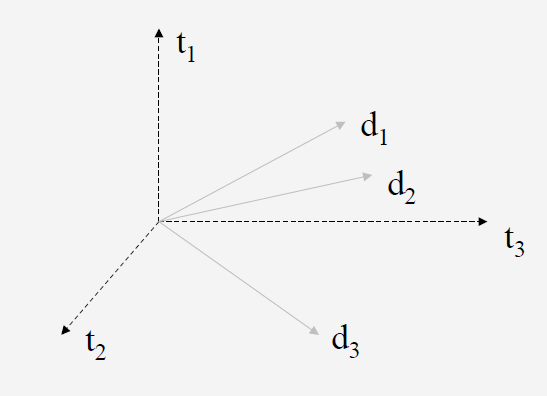
\includegraphics[width=4in] {fig_01.png}}
  \end{center}
  \caption{Representación de documentos en un espacio fectorial}
  \label{fig_01}
\end{figure}

En el contexto de evaluación automática de ensayos, se tiene un conjunto de documentos previamente evaluados por expertos humanos. Luego, para evaluar un texto nuevo, se calcula la similitud entre el documento nuevo y los documentos del corpus, y se asigna el puntaje del más similar, o una suma ponderada de los puntajes más similares.

La aplicación del método ha logrado una correlación con la evaluación realizada por humanos de 0.76 \cite{t5}. Sin embargo, la evaluación depende fuertemente de la co-ocurrencia de términos, por lo que un ensayo que sea sólo un conjunto de palabras sin una conexión clara, podría ser bien evaluado \cite{t9}. 

La efectividad del método depende de qué tan cercano es el cálculo de similitud realizado en el espacio vectorial, con la similitud real de los documentos. Algunos problemas que existen con este enfoque son los siguientes:

\begin{itemize}
	\item Polisemia ($sim(d_i, d_j) < cos(d_i, d_j)$): Si en el vocabulario definido para representar los vectores existen palabras que tengan múltiples significados, es posible que la similitud calculada (por ejemplo coseno), sobre-estime la similitud real entre los documentos, debido a que los términos se consideran equivalentes pues solo importa su frecuencia de aparición.
	\item Sinónimos ($sim(d_i, d_j) > cos(d_i, d_j)$): Dos documentos que sean similares en cuanto a contenido pero utilicen diferentes términos, entre ellos, sinónimos, se considerarán poco similares, pues el coseno del angulo dependerá de qué tan cercanos se encuentran en el espacio vectorial, es decir, se subestima la similaridad real que existe entre dos documentos.
	\item Relaciones: Los humanos son capaces de establecer relaciones entre palabras, debido a que un lector tiene una representación mental y conceptual de las mismas, cada palabra tiene un significado (por ejemplo existen relaciones entre las palabras doctor/paciente/enfermera/tratamiento). El modelo de espacio vectorial no logra detectar estas relaciones.
	\item Se tiene una matriz muy dispersa, pues los documentos se representan en un espacio altamente dimensional y es probable que haya términos que no ocurran en todos los documentos. Esto podría ocasionar problemas al realizar el cálculo de similitud, pues si existen demasiados elementos nulos, se podría subestimar la similitud real entre documentos, y si existe co-ocurrencia de muchos términos, se podría sobre-estimar la similitud real entre documentos.
\end{itemize}

Estos problemas traen como consecuencia la necesidad de tener métodos de reducción dimensional.

\section{Métodos de Reducción Dimensional}

\subsection{Análisis Semántico Latente}

Para abordar el problema de la co-ocurrencia de palabras, se ha aplicado una técnica de reducción dimensional conocida como {\em Análisis Semántico Latente} (LSA) \cite{t28}, la cual intenta extraer y representar el significado de las palabras, lo que permite encontrar similitudes entre documentos aunque no haya co-ocurrencia de términos. El método toma como supuesto que existen relaciones que subyacen de forma latente en la estructura semántica de los datos, y que se encuentran parcialmente ocultas. Este método requiere un corpus, y que se defina un vocabulario con las palabras más relevantes del corpus para representar los documentos en un espacio vectorial. El método considera un modelo de {\em bolsas de palabras} (BOW), es decir, asume que el orden de las palabras no importa. Posteriormente, se obtiene una matriz de palabras y documentos del corpus. Luego, se aplica una técnica matemática conocida como {\em descomposición de valores singulares} (SVD), para obtener una matriz reducida que en este contexto se denomina {\em espacio semántico}. Las dimensiones de este espacio semántico son una combinación lineal de documentos, las que se interpretan como {\em conceptos}, y posteriormente se puede definir una medida de similitud entre ellos. Luego, se puede medir la coherencia textual \cite{t8} \cite{t10} \cite{t20} \cite{t29}, y evaluar ensayos \cite{t9}. 

La evaluación de ensayos en LSA se realiza en dos etapas. En la primera etapa se requiere un corpus que contenga documentos relacionados al tópico a evaluar. Luego, se aplica LSA para obtener un espacio semántico. En la segunda etapa, se consideran ensayos pre-evaluados por humanos, y se comparan con ensayos nuevos utilizando algún criterio de similitud (por ejemplo coseno). Esta comparación se realiza dentro del espacio semántico obtenido en la etapa 1 \cite{t10}. Finalmente, al ensayo se le asigna la nota del ensayo más similar dentro del espacio semántico.

Un problema con LSA es que al utilizar un modelo de bolsa de palabras no considera el orden de las mismas. Por ejemplo se consideraría equivalente ``literatura fantástica'' con ``fantástica literatura''. El método tampoco considera la forma en que están escritas las oraciones, ya que  un texto podría ser bien evaluado si cumple con los criterios de similaridad. Por otro lado, LSA tiene problemas con la polisemia (palabras que tienen distintos significados), y ello afecta al momento de encontrar similitud entre dos documentos, pues dos documentos pueden utilizar una misma palabra pero hablar de temas diferentes. Otro problema ocurre con la elección de la dimensionalidad del espacio semántico, la cual se realiza utilizando heurísticas {\em ad-hoc}, por ejemplo se dice que se obtienen buenos resultados si se reduce la dimensionalidad a valores entre 100-300 \cite{t10}.

Para abordar parcialmente el problema relacionado al orden de las palabras, se ha propuesto una variación de LSA denominada {\em Generalized Latent Semantic Analysis} (GLSA) \cite{t13}. Este método utiliza frecuencia de n-gramas en lugar de palabras, lo que permite distinguir segmentos de texto como por ejemplo ``dióxido de carbono'' con ``Carbono de dióxido'', lo que LSA convencional consideraría como equivalente. Para la evaluación automática de ensayos, se realiza el mismo procedimiento que LSA, por lo que la única diferencia entre ambos métodos es el espacio semántico obtenido. En LSA se obtienen conceptos como combinación lineal de los vectores que representan las palabras, mientras que en GLSA son combinaciones lineales de vectores de n-gramas. Experimentalmente se ha obtenido una correlación 0.88 entre el puntaje asignado por humanos y el asignado por el método \cite{t13}. Algunos problemas de esta técnica incluyen:

\begin{itemize}
	\item Alta dimensionalidad del espacio vectorial debido a los n-gramas.
	\item Alto grado de dispersión, pues la co-ocurrencia de n-gramas es menos probable que la de palabras. Esta dispersión puede producir errores numéricos al aplicar descomposición de valores singulares.
	\item La descomposición de valores singulares es costosa computacionalmente y el costo crece exponencialmente dependiendo de los n-gramas a utilizar.
\end{itemize}

El problema de la polisemia no es totalmente resuelto por GLSA, ya que depende de la distribución de n-gramas utilizados para capturar el contexto en que la palabra fue utilizada. Por otro lado, GLSA tampoco tiene una base estadística sólida (no define un modelo generativo de los datos) lo que dificulta interpretar el espacio semántico obtenido. 

\section{Probabilistic Latent Semantic Analysis}

Para abordar los problemas mencionados previamente se ha propuesto un método probabilístico denominado {\em Probabilistic Latent Semantic Analysis} \cite{t41}, el cual considera que los datos pueden expresarse en términos de 3 tipos de variables:

\begin{itemize}
	\item Documentos: Los documentos del corpus a utilizar.
	\item Palabras: El vocabulario a considerar en el corpus.
	\item Tópicos: Variables ocultas.
\end{itemize}

PLSA se fundamenta en un modelo probabilístico denominado {\em Aspect Model}, el cual expresa que las variables ocultas (tópicos) están asociadas a las variables observadas (documentos y palabras). En la figura \ref{figura_plsa} se muestra una representación gráfica del modelo, en la que se describe el proceso generativo de N documentos en el corpus. $N_w$ es la cantidad de palabras en el documento $d$. Cada palabra $w$ tiene asociada un tópico $z$ (variable latente) que la genera.

\begin{figure}[!htbp]
  \begin{center}
    \leavevmode
    \fbox{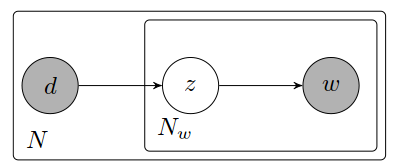
\includegraphics[width=3in] {figure_plsa.png}}
  \end{center}
  \caption{Representación gráfica de PLSA.}
  \label{figura_plsa}
\end{figure}

Las ventajas que posee PLSA respecto a LSA incluyen:

\begin{itemize}
	\item Modelo con base estadística sólida, donde los parámetros están bien definidos y tienen interpretación probabilística clara (variables latentes como tópicos), a diferencia de LSA donde el espacio semántico no tiene una interpretación clara. 
	\item Al estar basado en un enfoque probabilístico se puede utilizar teoría estadística para la selección del modelo (cantidad de tópicos a considerar, es decir, la dimensionalidad del espacio semántico), a diferencia de LSA donde se hace con heurísticas {\em ad-hoc}.
	\item Logra solventar el problema de la polisemia, pues se tienen grupos de palabras que representan un determinado tópico (variable oculta).
\end{itemize}

Este método se ha utilizado para la evaluación automática de ensayos, los resultados obtenidos son similares a los de LSA en conjuntos de datos pequeños, y mejores que LSA en corpus con más documentos.

\section{Métodos Basados en Bases de Conocimiento}
En general, los métodos basados en modelos de espacio vectorial tienen el problema de que no son capaces de detectar errores semánticos, como por ejemplo hechos contradictorios dentro de un texto, o hechos inconsistentes dentro del dominio en el que se quiere evaluar el texto. Debido a esto, se ha propuesto el uso de ontologías para la detección de errores semánticos \cite{t43}. Una ontología es una definición formal de tipos, propiedades, y relaciones entre entidades con respecto a un dominio específico. Básicamente, contiene axiomas que representan el dominio y sus características. Para evaluar la coherencia textual en un dominio específico, lo que se hace es crear una base de conocimiento que tenga axiomas sobre el dominio a considerar. Luego, para evaluar un texto, se genera una representación lógica del contenido del mismo y se evalúa la consistencia de los hechos mencionados en el texto con respecto a la base de conocimiento del dominio. Cualquier hecho que sea incosistente se considerará como un error semántico. Se ha encontrado que este método puede detectar errores semánticos que pasan desapercibidos en métodos basados en un modelo de espacio vectorial como LSA \cite{t44}. Un problema con este método es que la generación de la ontología y los axiomas se hace manualmente, por lo que se vuelve poco práctico si se tiene un corpus con miles de documentos. En los experimentos reportados se utilizan conjuntos de datos del orden de los 30 - 50 documentos.

\section{Coherencia Textual y Análisis de Discurso}
Los métodos mencionados previamente utilizan modelos de bolsa de palabras, es decir, el orden de las mismas no influye. Se ha demostrado que la coherencia textual está relacionada con el orden en que se presentan las ideas en un texto \cite{t33}. Existen métodos para medir coherencia textual que consideran la sintaxis de un texto \cite{t34} \cite{t35} y se fundamentan en la {\em teoría de centrado} \cite{t36}. Esta establece que un discurso está conformado por segmentos de texto y que cada segmento de texto está conformado por expresiones o enunciados ({\em utterances} $U_i$ - $U_n$). Cada expresión ($U_i$) tiene asociada un conjunto de entidades de discurso o centros del discurso (los cuales pueden ser nombres, pronombres, objetos, etc.), el cual se denomina {\em forward looking centers} $C_f(U_i)$. Los elementos de $C_f$ se rankean de acuerdo a su importancia dentro del discurso. El centro de $C_f$ que tiene el mayor rango se denomina $C_p$ o el centro preferido. También se define un centro que relaciona la expresión actual con la anterior, y se denomina {\em backward looking center} $C_b$, y se define como el centro con mayor rango en la expresión previa $U_{i-1}$ que es mencionado en la exprsesión $U_i$. $C_b$ es un tipo especial de centro ya representa el tema que está tratando $U_i$.

La teoría define cuatro tipos de transiciones, las cuales se muestran en la tabla \ref{t1}.

\begin{table}[!htbp]
\centering
\caption{Tabla de transiciones en la Teoría del Centrado}
\label{t1}
\begin{tabular}{lll}
\hline
\hline
                        & $C_b(U_i)=C_b(U_{i-1})$\_ & $C_b(U_i)\neq C_b(U_{i-1})$ \\
\hline
$C_b(U_i)=C_p(U_i)$     & {\em Continue}          & {\em Smooth Shift}        \\
$C_b(U_i)\neq C_p(U_i)$ & {\em Retain}            & {\em Rough Shift}         \\
\hline
\hline   
\end{tabular}
\end{table}

Estas transiciones se utilizan para evaluar qué tan coherente es un texto, y tienen un orden de preferencia, el cual se define como: Una transición tipo {\em continue} se prefiere respecto a una tipo {\em retain} la cual se prefiere respecto a una tipo {\em smooth shift} la cual se prefiere respecto a una tipo {\em rough shift}. La idea fundamental es que discursos coherentes tienden a mantener un centro entre expresiones ({\em utterance}) mientras que textos poco coherentes tienden a hacer cambios bruscos de centros (entidades de discurso). Para entender la idea, se propone el siguiente ejemplo:

\begin{enumerate}
	\item Juan tenía un terrible dolor de cabeza. \\
	($C_b=?$ $C_f=Juan>Dolor de Cabeza$ ,$transicion=ninguna$)
	\item Cuando la reunión terminó\\
	($C_b=ninguno$ $C_f=Reunion$ ,$transicion=${\em Rough Shift})
	\item él corrió a la farmacia\\
	($C_b=ninguno$ $C_f=Juan$ ,$transicion=${\em Rough Shift})
\end{enumerate}

Observamos que el fragmento de discurso es complicado de leer, debido a que el foco en la segunda expresión cambia bruscamente, primero se hablaba de {\em Juan} y su {\em Dolor de Cabeza} y luego se habla sobre una {\em reunión}. Se observa que si se cambia el orden de las oraciones, se torna en un texto más coherente:

\begin{enumerate}
	\item Juan tenía un terrible dolor de cabeza. \\
	($C_b=?$ $C_f=Juan>Dolor de Cabeza$ ,$transicion=ninguna$)
	\item él corrió a la farmacia\\
	($C_b=Juan$ $C_f=Juan>Farmacia$ ,$transicion=${\em Continue})
	\item cuando la reunión terminó\\
	($C_b=ninguno$ $C_f=Reunion$ ,$transicion=${\em Rough Shift})
\end{enumerate}

En este caso es claro que {\em Juan corrió} a la {\em farmacia} una vez terminada la {\em reunión}.

Esta teoría ha sido utilizada para determinar la correlación entre la proporción de transiciones {\em Rough Shift} que ocurren en un discurso y el puntaje asignado por humanos a un texto. Se ha encontrado que mientras mayor sea esta proporción, los textos tienden a ser menos coherentes \cite{t45}. La principal ventaja, es que se considera la sintaxis del texto (el orden de las expresiones es relevante). La desventaja que tiene es que depende fuertemente de la precisión con la que se capturan las entidades de discurso y se identifican los conjuntos $C_f$. En \cite{t45} se utilizaron textos etiquetados por humanos para la extracción de centros de discurso, debido a que métodos automáticos tienen problemas al momento de identificar las coreferencias dentro del texto.

Otro método de evaluación basado en esta teoría, toma como supuesto que existen patrones que es más probable que aparezcan en discursos coherentes. Para detectar estos patrones, un texto se representa mediante una matriz de entidades. Un ejemplo de texto y su matriz de entidades se muestran en las figuras 1 y 2.
	
\begin{figure}[!htbp]
  \begin{center}
    \leavevmode
    \fbox{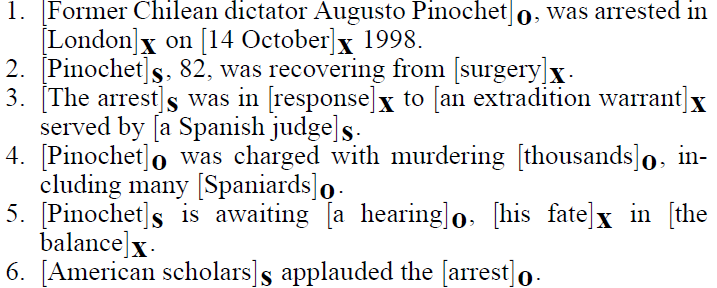
\includegraphics[width=4in] {figure_1.png}}
  \end{center}
  \caption{Texto con anotaciones sintácticas para el cálculo de matriz de entidades.}
  \label{figura1}
\end{figure}

\begin{figure}[!htbp]
  \begin{center}
    \leavevmode
    \fbox{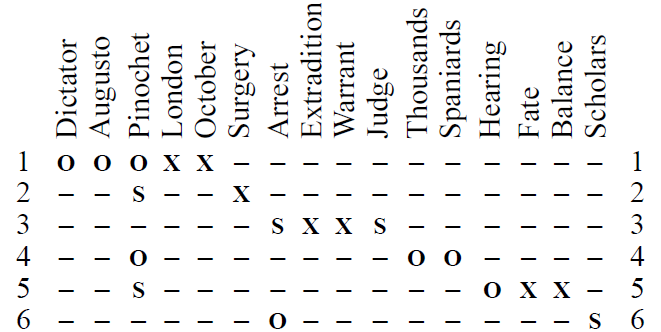
\includegraphics[width=4in] {figure_2.png}}
  \end{center}
  \caption{Una matriz de entidades}
  \label{figura2}
\end{figure}

Las columnas de la matriz representan la presencia o ausencia de una entidad en una secuencia de oraciones $(S_1,...,S_n)$. En particular, cada celda de la matriz representa el rol $r_{ij}$ de la entidad $e_j$ en la oración $S_i$. Los roles gramaticales reflejan si una entidad es un sujeto, objeto, ninguno o simplemente se encuentra ausente. Por ejemplo, en la figura 2, si se considera la entidad \textit{arrest} es un sujeto, en la oración 3, es un objeto en la oración 6, pero se encuentra ausente en el resto de las oraciones. 

Así, la coherencia de un texto $T(S_1, ..., S_n)$ con entidades $e1, ..., e_m$, se puede ver como una distribución de probabilidad conjunta que describe cómo las entidades están distribuidas a través de las oraciones del texto $T$:

\begin{equation}
	P_{coherence}(T) = P(e_1,...,e_m; S_1,...,S_n)
\end{equation}

Para generar este modelo de distribución, se requiere un conjunto de textos que los humanos consideren coherentes \cite{t36}. Luego, se puede predecir $P(e_1,...,e_m; S_1,...,S_n)$ en textos en los que se quiera evaluar la coherencia. Luego, $P_{coherence}(T)$ será mayor para textos que se consideren más coherentes que los que tengan un $P_{coherence}(T)$ menor.

El método también considera una componente semántica que modela la forma en que se conectan oraciones en términos de la representación mental que hace un lector al leer el texto. La cohesión léxica se representa a través de un modelo de {\em cadenas léxicas} \cite{t39}, es decir, secuencias de palabras relacionadas que abarcan una unidad textual (por ejemplo: oración, párrafo, etc.). De ahí que las unidades textuales coherentes deberán tener una alta concentración de estas cadenas, pues un texto coherente posee muchas palabras relacionadas semánticamente. Esto permite representar un texto sin considerar el orden de las palabras, luego, cada oración es un conjunto de palabras. Así, para medir la coherencia local de un texto se debe cuantificar la relación semántica entre oraciones adyacentes. Es decir, la coherencia de un texto $T$ se puede considerar como el promedio del grado de similaridad entre oraciones:

\begin{equation}
	coherencia(T) = \frac{\sum_{i=1}^{n-1}sim(S_i, S_{i+1})}{n-1}
	\label{eq5}
\end{equation}
Donde $sim(S_i, S_{i+1})$ es una medida de similaridad entre las oraciones $S_i$ y $S_{i+1}$.

Este método ha sido comparado con otros enfoques para medir coherencia textual (entre ellos LSA, basados en ontologías, basados en características superficiales) en el ámbito de resumenes generados automáticamente \cite{t33}. Los resultados muestran que no existe correlación entre los métodos, por lo que cada uno mide distintas componentes de la coherencia textual. Así, un modelo que considere estas componentes tendrá un mejor desempeño en términos de correlación con humanos que cualquier modelo por sí solo.

%%%%%%%%%%%%%%%%%%%%%%%%%%%%%%%%%%%%%%%%%%%%%%%%%%%%%%%%%%%%%%%%%%%%%%%%%%%%%%%%
% Step 12: Here's the main part of your research project. We can't tell
% you what to write here... that's your job.
% 
%%%%%%%%%%%%%%%%%%%%%%%%%%%%%%%%%%%%%%%%%%%%%%%%%%%%%%%%%%%%%%%%%%%%%%%%%%%%%%%%
\chapter{Método de Evaluación de Ensayos en base a Sintaxis y Semántica}\label{chap:contributions}

\chapter{Experimentos y Resultados}\label{chap:experiments}
%%%%%%%%%%%%%%%%%%%%%%%%%%%%%%%%%%%%%%%%%%%%%%%%%%%%%%%%%%%%%%%%%%%%%%%%%%%%%%%%
% Step 13: Add a conclusions chapter
%
% 
%%%%%%%%%%%%%%%%%%%%%%%%%%%%%%%%%%%%%%%%%%%%%%%%%%%%%%%%%%%%%%%%%%%%%%%%%%%%%%%%
\chapter{Conclusions}\label{chap:conclusion}

%%%%%%%%%%%%%%%%%%%%%%%%%%%%%%%%%%%%%%%%%%%%%%%%%%%%%%%%%%%%%%%%%%%%%%%%%%%%%%%%
% Step 14: Work out the bibliography
%
% 
%%%%%%%%%%%%%%%%%%%%%%%%%%%%%%%%%%%%%%%%%%%%%%%%%%%%%%%%%%%%%%%%%%%%%%%%%%%%%%%%
% Tips: 
%
% For named.bst, if I add a~\cite*{} it will add all the references I
% have in the bibliography file (whether they are referenced in the
% document or not)
%%%%%%%%%%%%%%%%%%%%%%%%%%%%%%%%%%%%%%%%%%%%%%%%%%%%%%%%%%%%%%%%%%%%%%%%%%%%%%%%
\bibliographystyle{plain}
\begin{thebibliography} {}
	\bibitem{t0}
	S. Valenti, F. Neri, and A. Cucchiarelli, ``An overview of current research on automated essay grading,'' {\em Journal of Information Technology Education}, vol. 2, pp. 319-330, 2003.
	
	\bibitem{t1}
	T. Miller, ``Essay assessment with latent semantic analysis,'' {\em Department of Computer Science, University of Toronto}, Toronto, ON M55 3G4, Canada, 2002.
	
	\bibitem{t2}
	L. M. Rudner and T. Liang, ``Automated essay scoring using Bayes' Theorem,'' {\em The Journal of Technology, Learning, and Assessment}, vol. 1, no. 2, 2002.
	
	\bibitem{t3}
	K.M Nahar and L.M. Alsmadi, ``The automatic grading for online exams in Arabic with essay questions using statistical and computational linguistics techniques,'' {\em MASAUM Journal of Computing}, vol. 1, no. 2, 2009.
	
	\bibitem{t4}
	S Ghosh and S. S. Fatima, ``Design of an Automated Essay Grading (AEG) system in Indian context,'' in {\em Proceedings of TENCON 2008-2008 IEEE Region 10 Conference}, pp. 1-6.
	
	\bibitem{t5}
	Y. Attali, J. Burstein, ``Automated essay scoring with e-rater,'' {\em The Journal of Technology, Learning and Assessment}, vol. 4, no.3, 2006.
	
	\bibitem{t6}
	L.M. Rudner, V. Garcia, C.Welch, ``An evaluation of the IntelliMetric essay scoring system,'' {\em The Journal of of Technology Learning, and Assessment}, vol. 4, no. 4, pp. 1-22, 2006.
	
	\bibitem{t7}
	P. W. Foltz, D. Laham, T.K. Landauer, ``Automated essay scoring: applications to educational technology,'' in {\em Proceedings of World Conference on Educational Multimedia, Hypermedia and Telecommunications}, 1999, pp.939-944.
	
	\bibitem{t8}
	B. Lemaire, P. Dessus, ``A system to assess the semantic content of student essay,'' {\em The Journal of Educational Computing Research},'' vol. 24, no. 3, pp. 305-320, 2001.
	
	\bibitem{t9}
	M.A. Hearst, ``The debate on automated essay grading,'' {\em Intelligent Systems and their Applications}, IEEE , vol.15, no.5, pp.22-37, Sept.-Oct. 2000.
	
	\bibitem{t10}
	T. Kakkonen, N. Myller, E. Sutinen, J. Timonen, ``Comparison of Dimension Reduction Methods for Automated Essay Grading,'' {\em Educational Technology and Society}, 2006, pp. 275-288.
	
	\bibitem{t11}
	 P. Selvi, N.P. Gopalan, ``Automated writing Assessment of Student's Open-ended Answers Using the Combination of Novel Approach and Latent Semantic Analysis,'' {\em Advanced Computing and Communications} ADCOM 2006. International Conference on , vol., no., pp.370-375, 20-23 Dec. 2006.
	
	\bibitem{t12}
	G. Russo-Lassner, J. Lin, P. Resnik, ``A Paraphrase-Based Approach to Machine Translation Evaluation,'' {\em Technical Report} LAMP-TR-125/CS-TR-4754/UMIACS-TR-2005-57, University of Maryland, College Park, August 2005.
	
	\bibitem{t13}
	M.M. Islam, A.S.M.L. Hoque, ``Automated essay scoring using Generalized Latent Semantic Analysis,'' {\em Computer and Information Technology (ICCIT)}, 13th International Conference on, pp.358-363, 2010.
	
	\bibitem{t14}
	H. Chen, B. He, T. Luo, B. Li, ``A Ranked-Based Learning Approach to Automated Essay Scoring,'' {\em Cloud and Green Computing (CGC)}, Second International Conference on, pp.448-455, 1-3 Nov. 2012.
	
	\bibitem{t15}
	C.D. Manning, H, Schutze, ``Foundations of Statistical Natural Language Processing,'' Cambridge, MA: MIT Press, 1990.
	
	\bibitem{t16}
	L. Rudner, L. Tahung, ``Automated Essay Scoring using Bayes' Theorem,'' {\em The Journal of Technology, Learning, and Assessments}, 3-21, 2002.
	
	\bibitem{t17}
	H. Breland, R. Jones, Laura J., ``The College Board Vocabulary Study,'' {\em College Entrance Examination Board}, New York, 1994.
	
	\bibitem{t18}
	C. Moncayo, F. Julio. ``La terminología como elemento de cohesión en los textos de especialidad del discurso económico-financiero'', Tesis Doctoral, Facultad de Filosofía y Letras, Universidad de Valladolid, pp. 1-50, 2002.
	
	\bibitem{t19}
	
	McCarthy, Philip M.; Briner, Stephen W.; Rus, Vasile y McNamara, Danielle S. ``Textual Signatures: Identifying Text-Types Using Latent Semantic Analysis to Measure the Cohesion of Text Structures'', Institute for Intelligent Systems, University of Memphis, USA., pp. 1-15, 2005.
	
	\bibitem{t20}
	E. Kintsch, D. Steinhart, G. Stahl, and the LSA Research Group, Developing Summarization Skills through the Use of LSA-Based Feedback, Interactive Learning Environments, 8:2, pp. 87-109, 2000.
	
	\bibitem{t21} Organización para el Desarrollo Económico (OECD). ``Informe sobre los resultados de los estudiantes chilenos en el estudio PISA 2012'', pp. 60-78, 2012. Unidad de Curriculum y Evaluación, Ministerio de Educación, Chile.

	\bibitem{t22} Fernández, Aguistín. ``Aprender a Leer: una tarea de todos y de siempre'', en Revista Digital
Umbral 2000, tomo 13, pp. 1-10, 2003.

	\bibitem{t23} Rivera Lam, Mailing. ``Estrategias de lecturas para la comprensión de textos escritos: El pensamiento reflexivo y no lineal en alumnos de educación superior'', en Revista Digital Umbral 2000, tomo 12, pp. 1-14, 2003.
	
	\bibitem{t24} Chung, Gregory K.W.K., and Eva L. Baker (2003). ``Issues in the Reliability and Validity of Automated Scoring of Constructed Responses'', p. 23. In: Automated Essay Scoring: A Cross-Disciplinary Perspective. Shermis, Mark D., and Jill Burstein, eds. Lawrence Erlbaum Associates, Mahwah, New Jersey, ISBN 0805839739.
	
	\bibitem{t25} Dikli, Semire (2006). ``An Overview of Automated Scoring of Essays''. Journal of Technology, Learning, and Assessment, 5.
	
	\bibitem{t26} Christopher D. Manning, Prabhakar Raghavan and Hinrich Schütze, ``Introduction to Information Retrieval'', Cambridge University Press. 2008.
	
	\bibitem{t27} Daniel Jurafsky and James H. Martin, ``An Introduction to Natural Language Processing, 
Computational Linguistics, and Speech Recognition'', Second Edition. 2009.

	\bibitem{t28} T. Landauer, S. Dumais, ``Introduction to Latent Semantic Analysis'', in: Discourse Procesess 25, pp. 259-284, 1997.
	
	\bibitem{t29} S. Hernández, A. Ferreira, ``Evaluación Automática de Coherencia Textual en Noticias Policiales Utilizando Análisis Semántico Latente'', Revista de Lingüística Teórica y Aplicada. Concepción (Chile), 48 (2), II Sem. 2010, pp. 115-139.
	
	\bibitem{t30} F. Wild, ``Parameters Driving Effectiveness of Automated Essay Scoring with LSA'', IN: Proceedings of the 9th CAA Conference, Loughborough: Loughborough University.
	
	\bibitem{t31} Mehryar Mohri, Afshin Rostamizadeh, Ameet Talwalkar (2012). ``Foundations of Machine Learning,'' The MIT Press. ISBN 978-0-262-01825-8.
	
	\bibitem{t32} Grosz, Barbara J, Pollack, Martha E. y Sidner, Candace L., ``The Discourse'', The MIT
Press, pp. 437-467, 1989.

	\bibitem{t33} M. Lapata and R. Barzilay, ``Automatic evaluation of text coherence: models and representations,'' In Proceedings of the 19th international joint conference on Artificial intelligence (IJCAI 05). Morgan Kaufmann Publishers Inc., San Francisco, CA, USA, 1085-1090.
	
	\bibitem{t34} Laura Alonso i Alemany and Maria Fuentes Fort, ``Integrating cohesion and coherence for automatic summarization.'' In Proceedings of the tenth conference on European chapter of the Association for Computational Linguistics - Volume 2 (EACL 03), Vol. 2. Association for Computational Linguistics, Stroudsburg, PA, USA, 1-8. 
	
	\bibitem{t35} Ani Nenkova, Rebecca Passonneau, and Kathleen McKeown, ``The Pyramid Method: Incorporating human content selection variation in summarization evaluation,'' ACM Trans. Speech Lang. Process. 4, 2, Article 4 (May 2007)
	
	\bibitem{t36} B. Grosz, A. Joshi, S. Weinstein, ``Centering: A framework for modeling the local coherence of a discourse,'' Computational Linguistics, pp. 203-225.
	
	\bibitem{t37} Yen-Yu Chen, Chien-Liang Liu, Tao-Hsing Chang, Chia-Hoang Lee, ``An Unsupervised Automated Essay Scoring System,'' in Intelligent Systems, IEEE , vol.25, no.5, pp.61-67, Sept.-Oct. 2010.
	
	\bibitem{t38} M. Collins, ``Head-driven Statistical Models for Natural Language Parsing,'' PhD thesis, University of Pennsylvania, 1998.
	
	\bibitem{t39} J. Morris and G. Hirst, ``Lexical cohesion computed by thesaural relations as an indicator of the structure of text. Computational Linguistics, 1(17):21-43, 1991.
	
	\bibitem{t40} K. Zupanc, Z. Bosnic, ``Automated Essay Evaluation Augmented with Semantic Coherence Measures,'' in Data Mining (ICDM), 2014 IEEE International Conference on , vol., no., pp.1133-1138, 14-17 Dec. 2014
	
	\bibitem{t41} T. Hoffman, ``Unsupervised learning by probabilistic latent semantic analysis'', Machine Learning, 42 (1-2), pp. 177-196, 2001.
	
	\bibitem{t42} T. Kakkonen, N. Myller, E. Sutinen, J. Timonen, ``Comparison of Dimension Reduction Methods for Automated Essay Grading,'' Educational Technology and Society, pp. 275-288, 2008.
	
	\bibitem{t43} F. Gutierrez, D. Dou, S. Fickas, G. Griffiths, ``Online Reasoning for Ontology-Based Error Detection in Text'', OTM 2014, LNCS 8841, pp. 562-579, 2014.
	
	\bibitem{t44} F. Gutierrez, D. Dou, S. Fickas, G. Griffiths, ``Providing Grades and Feedback for Student Summaries by Ontology-based Information Extraction,'' CIKM\' 12, 2012.
	\bibitem{t45} E. Miltasaki, K. Kukich, ``Evaluation of text coherence for electronic essay scoring systems,''. Natural Language Engineering, 2004.
	
	\bibitem{t46} W. H. ``Dubay, Smart Language: Readers , Readability , and the
Grading of Text''. BookSurge Publishing, 2007.

	\bibitem{t47} C. Smith and A. Jönsson, ``Automatic Summarization As Means Of Simplifying Texts, An Evaluation For Swedish'', in Proceedings of the 18th Nordic Conference of Computational Linguistics NODALIDA 2011, B. Sandford Pedersen, G. Nespore, and I. Skadina, Eds., 2011, pp. 198?205.

	\bibitem{t48} A. Mellor, ``Essay Length , Lexical Diversity and Automatic Essay Scoring,'' Memoirs of the Osaka Institute of Technology, vol. 55, no. 2, pp. 1?14, 2011.
	
	\bibitem{t49} Y. Attali, ``A Differential Word Use Measure for Content Analysis in Automated Essay Scoring,'' ETS Research Report Series, vol. 36, 2011.
	
	\bibitem{t50} R. Barzilay, M. Lapata, ``Modeling Local Coherence: An Entity-based Approach,'' Procedings of the 43rd Annual Meeting of the ACL, pp. 141-148, 2005.
	
	\bibitem{t51} T. Mikolov, K. Chen, G. Corrado, D. Jeffrey, ``Efficient estimation of word representations in vector space,'' arXiv preprint arXiv:1301.3781, 2013a.

\end{thebibliography}

\end{document}
